% Chapter 3

\chapter{Related Works} % Main chapter title

\label{Chapter2} % For referencing the chapter elsewhere, use \ref{Chapter1} 

\lhead{Chapter 2. \emph{Related Works}} % This is for the header on each page - perhaps a shortened title

%----------------------------------------------------------------------------------------

This section provide an overview of the existing instances of static
energy maps and dynamic energy maps. \sref{staticEnergyMap} and
\sref{dynamicMap} presents a general information of the energy mapping
instanceses. Then the summary of demand side information, supply side
information and techniques used to produce these Static and Dynamic
Energy Map instances are shown in \sref{summaryMap}.

\section{Static Energy Map}\label{staticEnergyMap}
\subsection{London Heat Map}
Under the goal of supplying 25\% of the total energy with
decentralized energy (DE) by the year 2025, the Decentralised Energy
Master Planning Program (DEMaP) was conducted between 2008 to 2010 to
``identify opportunities for district heating networks through heat
mapping and energy masterplanning''~\cite{londonHeatMap}. In this
study, the term DE only refers to ``combined heat and power systems
connected to district heating
networks''~\cite{decentralHeatMap2011}. 

London Heat Map is a publicly accessible interactive map developed as
part of the DEMaP project. It is completed for the London Boroughs in
2012. It can act as a starting point of Energy Master Plan for local
authorities, and can assist developers to make connections to existing
DE networks to meet policy requirements (London Plan DE
policy)~\cite{decentralHeatMap2011, londonHeatMap}. Point features of
high heating energy consumers and suppliers, existing and emerging
energy networks are depicted on the interactive map. High DE potential
regions (``focus area''~\cite{decentralHeatMap2011}) are identified
and depicted on the map to highlight the opportunities of utilizing
the heat supply in the community planning and development
(\fref{fig:londonHeat}). The ``live-database'' property of London Heat
Map allows new data of energy consumption be uploaded by users.

The criteria applied for identifying focus area include: 1) near to
existing or emerging DE network, 2) high heat demand density 3) anchor
load building, 4) diverse heating demand profile 5) has public
ownership with policy concerns to make connections to the DE
network~\cite{decentralHeatMap2011}. The physical constraint are also
considered in finalizing the high DE potential regions.

\begin{figure}[h!]
  \centering
  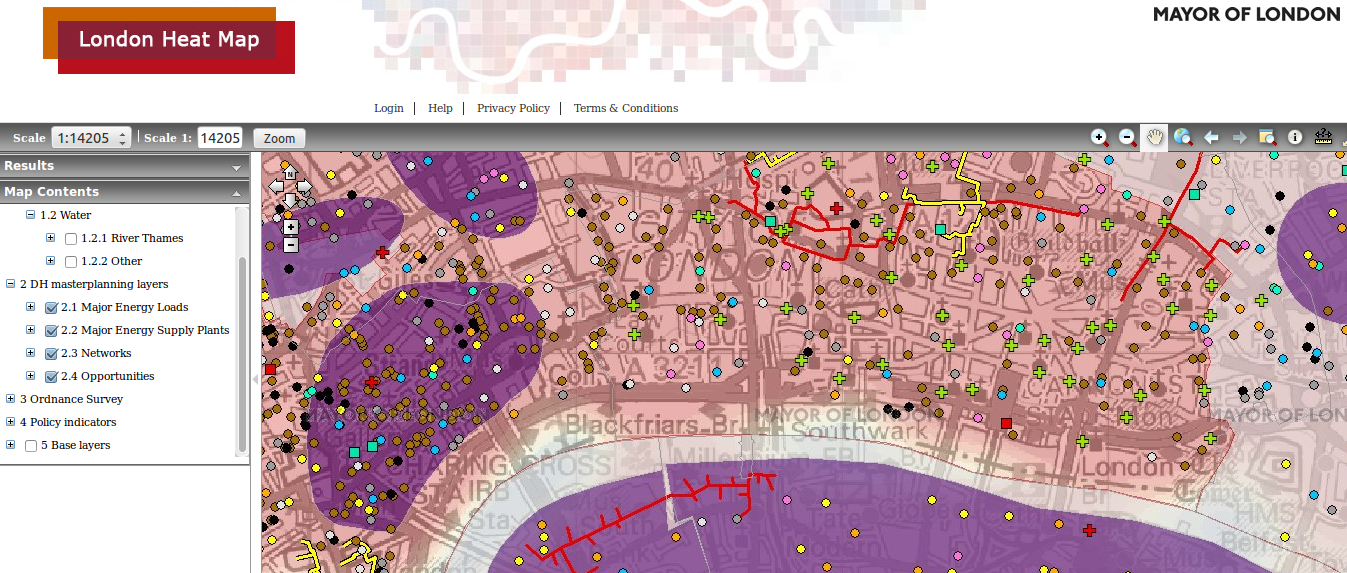
\includegraphics[width=0.7\linewidth]{londonHeat.png}
  \caption[London Heat Map]{London Heat Map~\cite{londonHeatMapMap}}
  \label{fig:londonHeat}
\end{figure}

\subsection{National Heat Map}
National Heat Map (\fref{fig:nhm}) is another UK energy mapping
project that focuses more on the industry
side~\cite{decentralHeatMap2011}. It is a ``high resolution
web-based'' heating energy interactive map, developed by the
Department of Energy and Climate Change (DECC). It aims at ``support
planning and deployment of local low-carbon energy projects in
England''~\cite{heatMap2015}. Power plant developers can use this map
to consider the feasibility for a CHP plant under policy
requirements~\cite{decentralHeatMap2011}. Heating demand density
($kWh/m^2$) of four major building sectors: public buildings,
commercial buildings, industry buildings and residential buildings,
together with the total demand is plotted on the map as a 2D raster
image with a discrete color scheme from blue to red representing low
to high heating demand. Heat source of CHP stations and thermal power
stations are plotted as point features in the map. Address level heat
demand data in csv format is also available for local authorities upon
request~\cite{heatMapLocal2012}.

\begin{figure}[h!]
  \centering
  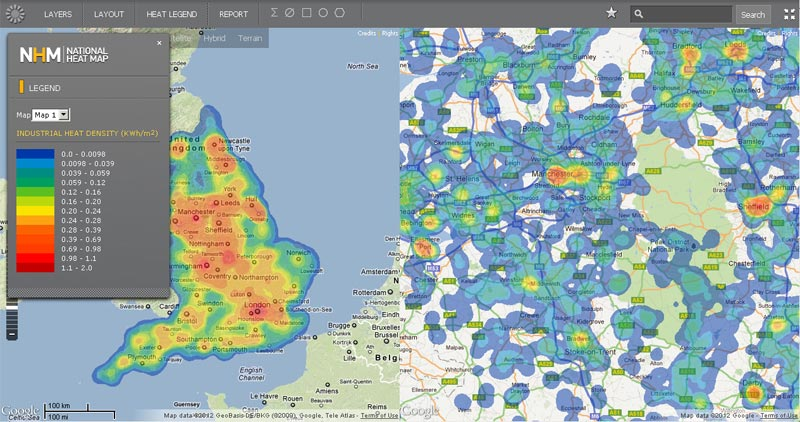
\includegraphics[width=0.5\linewidth]{nhm.jpeg}
  \caption[National Heat Map]{National Heat Map~\cite{heatMap2012}}
  \label{fig:nhm}
\end{figure}

\subsection{Water Source Heat Map}
The ``Water Source Heat Map'' (\fref{fig:waterMap}) is an added layer
group to the existing National Heat Map with information about the the
heat potential of the 4041 waterways in England. Heat potential of
waterways are represented in temperature, surface area, flow rate and
heat capacity ($kJ/m^3$ for coastal and estuary, $kW$ for canal, river
and settlement). It aims at supporting the plan of water-based thermal
system as water-based heat pump~\cite{waterHeatMap}. The map revealed
the large thermal capacity of water bodies that could serve over one
million buildings in the UK~\cite{waterHeatMap}.

\begin{figure}[h!]
  \centering
  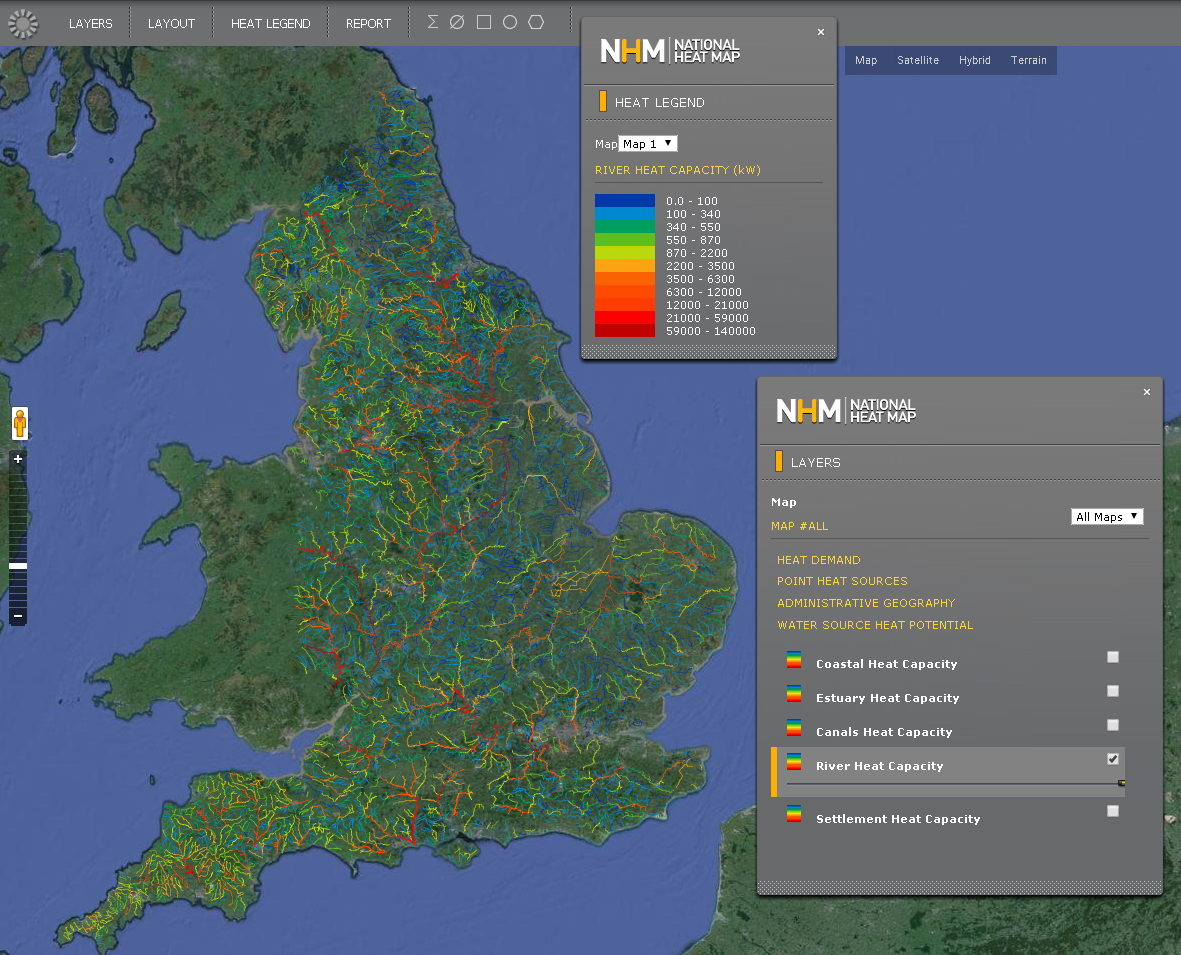
\includegraphics[width=0.5\linewidth]{waterMap.png}
  \caption[Water Heat Map]{Water Source Heat Map~\cite{waterHeatMap}}
  \label{fig:waterMap}
\end{figure}

\subsection{Calgary Energy Map}
One of the early instances of Static Energy Mapping is the Energy
Mapping Study of City of Calgary in 2008, carried out by Canadian
Urban Institute. It aims at providing insights to achieve the goal of
reducing 50\% of Green House Gas (GHG) emissions by
2050~\cite{aacip2009}. It depicts 1) how building design strategies
and land use planning can influence the city level energy use
intensity 2) the availability of alternative energy sources and the
opportunities to combine building level sustainable design technology
with the community level energy system design.

Calgary energy map first compares energy use intensity (the annual
total demand for thermal energy of space heating cooling, hot water
and electricity per unit area~\cite{aacip2009}) in GJ/ha between two
development cases: ``business as usual'' case and ``ultra-high
efficiency'' case (\fref{fig:calgaryCmp}). The comparison demonstrated
a 34\% reduction in energy use intensity from the former to the
latter~\cite{aacip2009}.

\begin{figure}[h!]
  \centering
  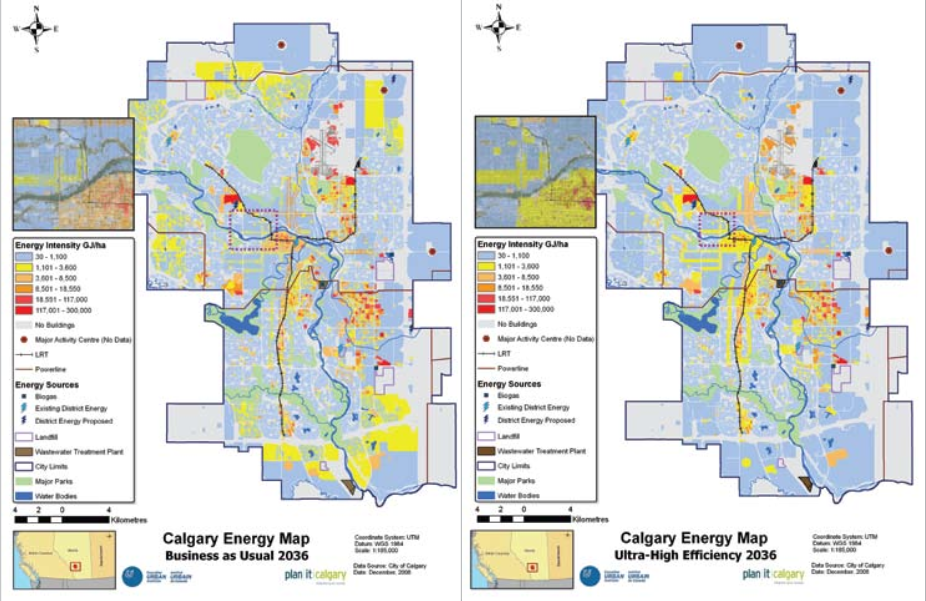
\includegraphics[width=0.6\linewidth]{calgaryCmp.png}
  \caption[Calgary Energy Demand Map]{Calgary Energy Map (Business as Usual, Ultra-High
    Efficiency)~\cite{aacip2009}}
  \label{fig:calgaryCmp}
\end{figure}

It also shows alternative energy sources of district energy, solar hot
water, solar air, energy sharing and PV installation on the map
(\fref{fig:calgaryAlter}). By overlaying the alternative technology
map and the ``ultra-high efficiency'' map, it highlights the
opportunities of using alternative renewable energy sources and
district energy system to further improve the energy performance of
high energy demand areas after high performance building design was
applied~\cite{aacip2009}.

\begin{figure}[h!]
  \centering
  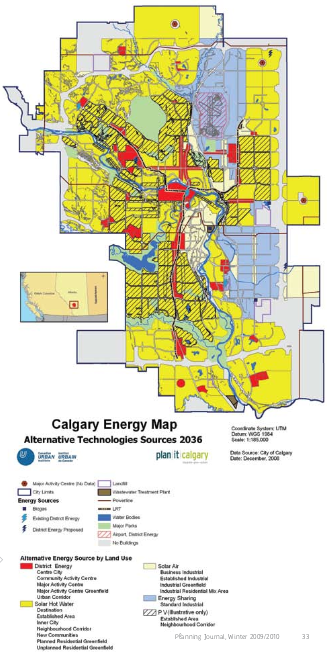
\includegraphics[width=0.3\linewidth]{calgaryAlter.png}
  \caption{Calgary Energy Map Alternative Energy Source~\cite{aacip2009}}
  \label{fig:calgaryAlter}
\end{figure}

\subsection{Energy Potential Mapping}
Dobbelsteen et al. described a framework of Energy Potential Mapping
(EPM) that aggregates information of energy supply, demand and
infrastructure on the same map with demand and supply represented in
the same unit of GJ or GJ/ha~\cite{Dobbelsteen2013}.

In 2010, a ``Heat Mapping'' study under the framework of EPM was
launched by TU Delft aiming at visualizing heat demand and supply and
infrastructure with the same unit that facilitates easy comparison and
facilitates the matching of supply and
demand~\cite{Dobbelsteen2013}. The map is presented with aggregated
supply and demand in a 3D Heat Map. The absolute quantity of each type
of demand and supply is represented with extruded height in the 3D
map. Demand is represented with a transparent 3D feature, and each
supply source is represented with solid 3D feature in a different
color~\cite{Dobbelsteen2013}.

\begin{figure}[htbp]
  \centering
  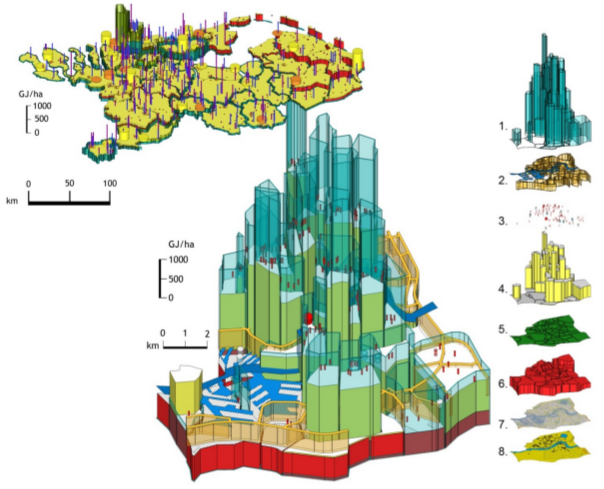
\includegraphics[width=0.7\linewidth]{heatmapNL.png}
  \caption[Rotterdam Heat Map]{Heat Mapping of Netherlands and
    Rotterdam~\cite{Dobbelsteen2013}}
  \label{fig:heatmapNL}
\end{figure}

\section{Dynamic Energy Map}\label{dynamicMap}
Per definition of Dynamic Energy Map in the introduction, there are
not instances that fully realized all the desired functions yet. In
this section, some valuable attempts towards realizing and exploring
the power of dynamic energy mapping will be discussed.

\subsection{Lower Hill District Dynamic Mapping Project}
In 2011 to 2012, the Dynamic Energy Map of the Lower Hill District,
Pittsburgh, PA was created. It is designed to conduct feasibility
analysis and comparison of alternative energy supply techniques of a
district energy system~\cite{baird2014, Ramesh2013}. A geo-data base
was created with ArcMap, ArcScene and Sketchup. In the database, each
building, represented as a 3D feature, contains attributes of its
building name, annual energy consumption, energy use intensity (EUI),
and annual and monthly peak demand. The map is online accessible via
GIS Cloud (\fref{fig:mellonArenaGIS}).

\begin{figure}[h!]
  \centering
  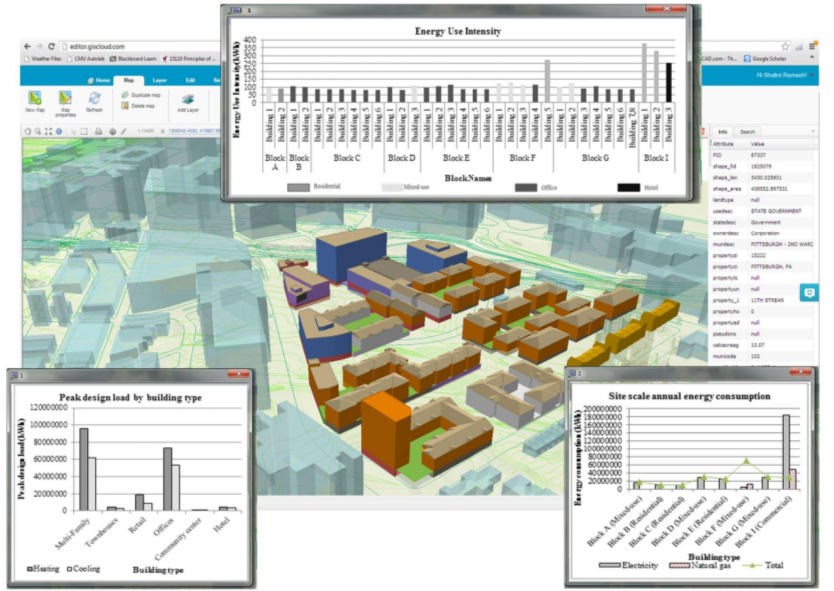
\includegraphics[width=0.7\linewidth]{mellonArenaGIS.png}
  \caption[Lower Hill District 3D GIS Map]{Online Accessible GIS-database with GIS
    Cloud~\cite{baird2014, Ramesh2013}}
  \label{fig:mellonArenaGIS}
\end{figure}

The feasibility analysis and temporal data display are separated from
the geo-database and is performed in a excel screening tool. The tool
takes input of energy cost rate, building type and size, development
phase and central plant types and feature and produces a feasibility
analysis and related temporal graphs (\fref{fig:3dexcel}) of annual
hourly energy consumption for each building type and the aggregated
demand of natural gas, cooling use electricity and total electricity.

\begin{figure}[h!]
  \centering
  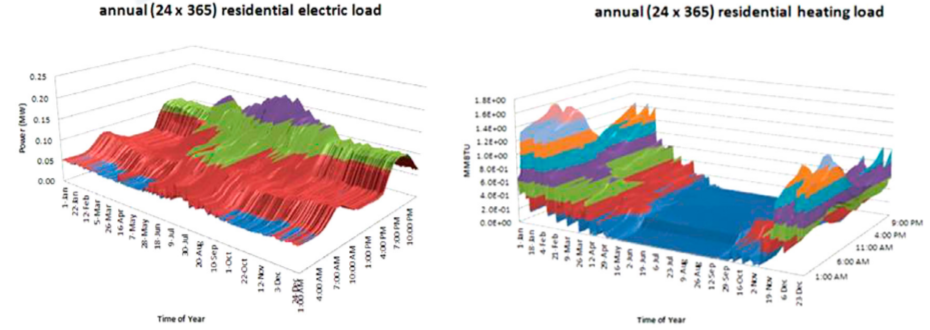
\includegraphics[width=0.7\linewidth]{3dexcel.png}
  \caption[Heating/Electricity Residential]{Heating Load and
    Electricity Load for Residencial Building~\cite{baird2014}}
  \label{fig:3dexcel}
\end{figure}

\subsection{Energy Mapping to Identify Opportunities for Future
  Networks Project (EMIOFN)}
Another instance of energy demand dynamic map with high spatial
resolution was found in the project ``Energy Mapping to Identify
Opportunities for Future Networks''~\cite{Diaz2013}. The aim of the
project is to ``analyze the spatial and temporal distribution of
energy consumption'' and support decision making and design of energy
network: more specifically, to identifiy opportunities of District
Heating, CHP plant development and Building Design
Improvement~\cite{Diaz2013}.

Energy Demand Maps of three different resolutions were created using
QGIS: campus level, community level and city level. Energy data was
retrieved from both metered data (used in campus level map) and HEM
simulation (used in community and city level map). HEM is a tool for
``mapping the possiblemapping the possible carbon and energy
performance of a dwelling. It has pre-simulated results embedded as a
data table in the tool and applies the appropriate system and context
calculations to provide instant energy, carbon and cost results''~\cite{HEMesru2015}.

For the campus level map, the heat demand density (heat demand over
conditioned area) were depicted to identify ``outliers'': the
buildings with high heat demand~\cite{Diaz2013campus}. These outliers
were potential buildings need to be improved in building insulation
level or HVAC system efficiency. They claim a spatial map is
sufficient for this outlier identification process
(\fref{fig:heatGlasgow}). They also created a temporal spatial map of
monthly heat consumption that is in the form of both small multiples
(\fref{fig:seqheatGlasgow}) and non-interactive animated map
(\fref{fig:animeheatGlasgow}). With the dynamic map, they identified
two campus buildings with high heat demand through the whole year
(anchor load building) and concluded that the two buildings could
connect to a district heating system. They also created two animated
maps with electricity and natural gas. By comparing these two animated
maps, consistent high consumers for electricity and gas were
identified as potential candidate building for a micro-CHP
system~\cite{microCHP}.

\begin{figure}[h!]
  \centering
  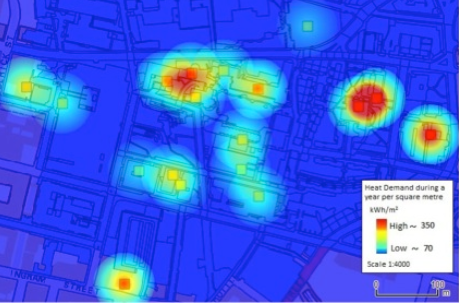
\includegraphics[width=0.5\linewidth]{heatGlasgow.png}
  \caption[Heat Demand Density]{Campus Level Heat Demand Density Map~\cite{Diaz2013campus}}
  \label{fig:heatGlasgow}
\end{figure}

\begin{figure}[h!]
  \centering
  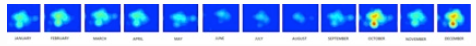
\includegraphics[width=0.5\linewidth]{seqheatGlasgow.png}
  \caption[Monthly Heat Demand (Small Multiple)]{Campus Level Monthly Heat Demand Map in Small Multiples\cite{Diaz2013campus}}
  \label{fig:seqheatGlasgow}
\end{figure}

\begin{figure}[h!]
  \centering
  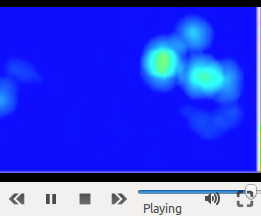
\includegraphics[width=0.3\linewidth]{animeheatGlasgow.png}
  \caption[Campus Animated Map]{Campus Level Monthly Heat Demand Map in Animation\cite{Diaz2013campus}}
  \label{fig:animeheatGlasgow}
\end{figure}

The community level spatial and temporal GIS analysis undertook a
similar process as the campus level except for the energy data is
retrieved from HEM simulation. By comparing the four different
building types: ``Traditional Build, New Build, Council Estate, High
Rise Flat'', they identified the consistent high gas and electricity
demand of High Rise Flat buildings. They also discovered that the
improvement of building design could adjust the heat to power ratio
(HTP) and could make applying CHP option feasible~\cite{Diaz2013com}.

\section{Summary}\label{summaryMap}
\subsection{Demand Side Information}\label{sec:demandInfo}
\tref{tab:demandInfo} summarizes the energy demand topics of the cases
presented in this section. The demand information presented in all
cases is heat demand except that the Calgary map has information of
the total energy demand: the sum of heating cooling and electricity
demand. The demand time resolution is year (represented as annual
total or annual total density) or month (monthly peak or monthly
total) for almost all instances, except that the Lower Hill District
Project screening tool has hourly demand information in the screening
tool.

\begin{table}[h!]
\centering
\caption{Demand Side Input Information}
\label{tab:demandInfo}
\begin{tabular}{p{3cm}|p{3cm}|p{3cm}|p{3cm}}
  \hline
  Project                 & Demand Topic                                             & Time                                        & Unit                      \\
  \hline
  \hline
  London Heat Map         & heat demand                                              & annual total density                                & kWh/m2 per year           \\
  \hline
  National Heat Map       & heat demand                                              & annual total density                                & kWh/m2 per year           \\
  \hline
  Water Source Heat Map   & x                                                        & x                                           & x                         \\
  \hline
  Calgary Map             & sum of space heating, cooling, hot water and electricity & annual total density                                & GJ/ha per year            \\
  \hline
  Dutch Heat Map          & heat demand                                              & annual total density                                & GJ/ha per year            \\
  \hline
  Lower Hill District Map & heat demand and electricity demand                       & Geo-database: annual total density, annual total and monthly peak & kBtu/ft$^2/year$ for EUI, kBtu for annual total, Btu/hr for peak demand \\ 
  \cline{3-4}
                          &                                                          & Screening tool: hourly                      & MW for electricity demand, MMBtu for heat demand     \\
  \hline
  EMIOFN                  & heating and cooling demand                                              & annual total density and monhly total              & kWh/m2 per year          \\
  \hline
\end{tabular}
\end{table}

The information included in my dynamic energy map is similar to that
of Calgary energy map: space heating, cooling, hot water and
electricity demand are depicted on the map. Calgary map has a single
layer of total demand, while my dynamic energy map provide single
layers of heating, cooling and electricity demand over time, as well
as two bivariate map layers: a bivariate layer of space heating and
cooling demand and a bivariate layer of heating demand and electricity
demand. The bivariate layer of space heating and cooling demand can
help users identify energy recovery opportunities
(\fref{fig:heatcool}). The bivariate layer of heat and power
accompanied with the aggregated heating and electricity data plot can
help users identify help the sizing of community district system CHP
plant(\fref{fig:heatpower}). Data plot of heating, cooling and
electricity of the community and single buildings in the community are
also provided to anchor quantitative information
(\fref{fig:heatCoolElec}).

\begin{figure}[h!]
  \centering
  \begin{subfigure}{0.4\textwidth}
  \centering
  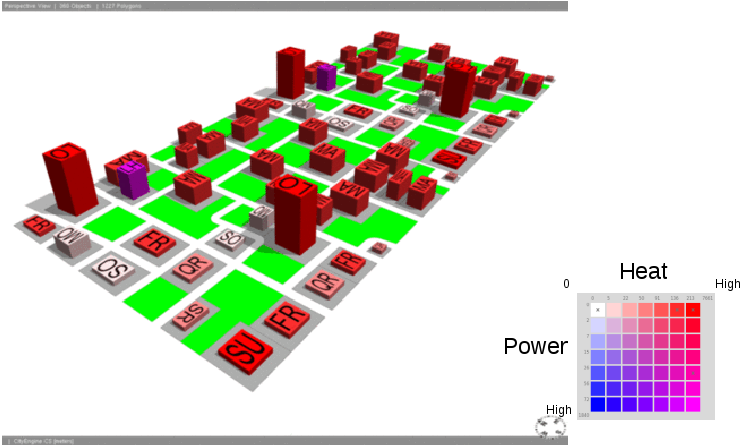
\includegraphics[width=\linewidth]{heatcool.png}
  \caption[Bivariate Layer of Heating and Cooling]{3D bivariate layer
    of space heating and space cooling demand}
  \label{fig:heatcool}
\end{subfigure}
~
\begin{subfigure}{0.4\textwidth}
  \centering
  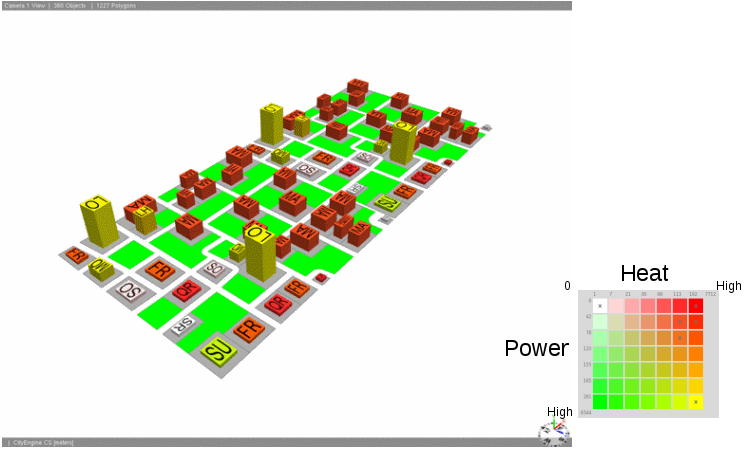
\includegraphics[width=\linewidth]{heatpower.png}
  \caption[Bivariate Layer of Heating and Electricity]{3D bivariate
    layer of heating and electricity demand}
  \label{fig:heatpower}
\end{subfigure}
\caption[Comparing Heating:Gas and Space Heating]{Comparing
  Heating:Gas and Space Heating}
\end{figure}

\begin{figure}[h!]
  \centering
  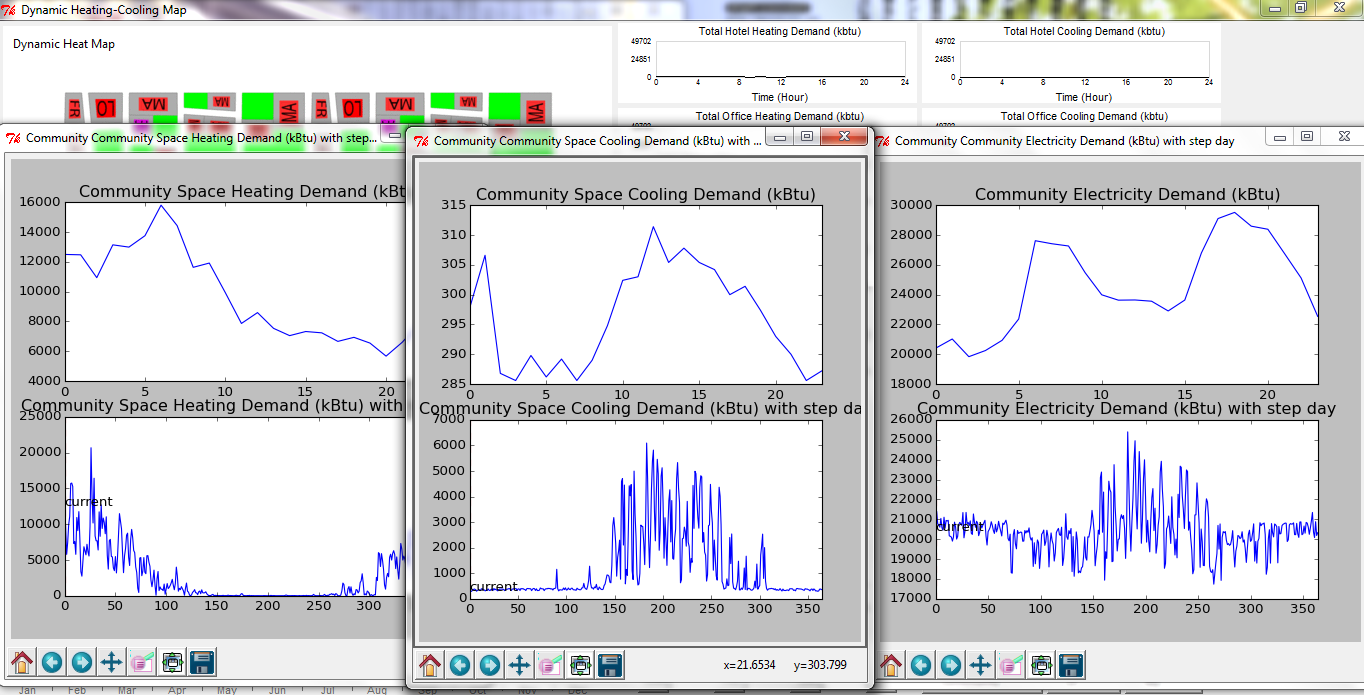
\includegraphics[width=0.5\linewidth]{heatCoolElec.png}
  \caption[Plot of Heating, Cooling and Electricity]{The example shows
    the plot of heating, cooling and electricity demand of the Large
    Office}
  \label{fig:heatCoolElec}
\end{figure}

Comparing with the static and dynamic map instances, which all use
annual / monthly total / total density as the indicator for energy
demand except that the screening tool in the Lower Hill District
Project has hourly demand information. My dynamic energy map adopts
the time resolution as the screening tool in the Lower Hill District
Project. It contains hourly energy demand data for every single
building and the community. Sizing of a district system requires peak
thermal energy demand of the community. This variable is missing from
all the existing static maps. My dynamic energy map shows the total
heat and electricity demand as plot on the interface and the users can
use this information to size a district energy system
(\fref{fig:CHPHeating}). 

% plot of aggregate demand (heating)
\begin{figure}[h!]
  \centering
  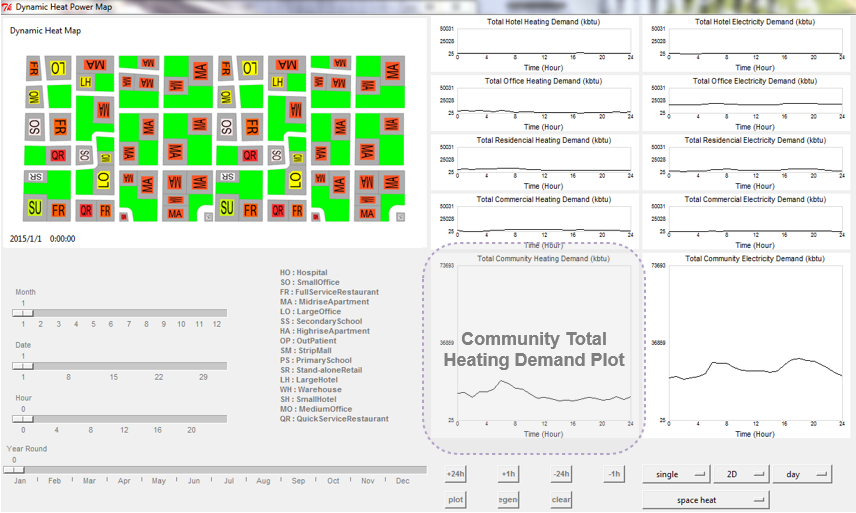
\includegraphics[width=0.7\linewidth]{CHPHeating.png}
  \caption[Plot of Heating, Cooling and Electricity]{Plot of Heating, Cooling and Electricity}
  \label{fig:CHPHeating}
\end{figure}

I chose to represent energy demand as absolute value rather than
density value in order to provide quantitative information for the
amount of energy that could be recovered within building groups or
communities and to provide information for the total thermal energy
demand in order to size system capacity of a CHP plant. 

My dynamic energy map also provide different forms of energy data
aggregation over the time dimension, such as total, peak and average
demand over a year, a month a week or a day (\fref{fig:aggOption}).
% plot of aggregate total, ave, peak etc.
\begin{figure}[h!]
  \centering
  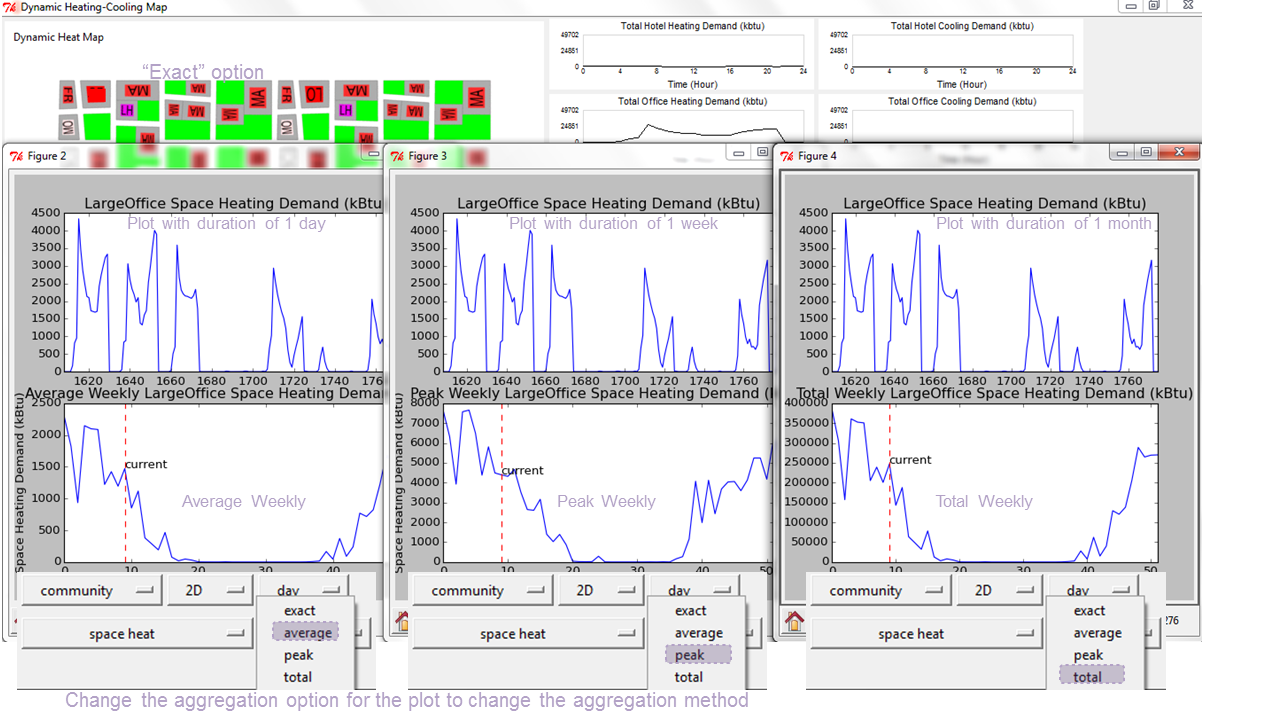
\includegraphics[width=0.7\linewidth]{aggOption.png}
  \caption[Plot of Different Energy Aggregation Method]{Plot of Different Energy Aggregation Method}
  \label{fig:aggOption}
\end{figure}

\subsection{Map Representation}\label{sec:mapRepre}
\tref{tab:mapRep} summarizes the data representation method used in
the cases presented in this section.

\begin{table}[h!]
\centering
\caption{Map Representation of Related Works}
\label{tab:mapRep}
\begin{tabular}{p{4cm}|p{4cm}|p{4cm}}
  \hline
  Project                 & Geometry                            & Quantity representation         \\
  \hline
  \hline
  London Heat Map         & point                               & graduated symbol size           \\
  \hline
  National Heat Map       & raster                              & discrete graduated color ramp (blue to red with red for high heat demand) \\
  \hline
  Water Source Heat Map   & x                                   & x                               \\
  \hline
  Calgary Map             & polygon                             & discrete graduated color ramp  (blue to red with red for high energy demand) \\
  \hline
  Dutch Heat Map          & extruded polygon                    & height of polygon               \\
  \hline
  Lower Hill District Map & Geo-database: 3D building and site  & Bar Chart                       \\
  \cline{2-3}
                          & Screen Tool: no geometry associated & Screening Tool: 3D height graph \\
  \hline
  EMIOFN                  & raster                              & continuous graduated color (blue to red with red for high heat demand) \\
  \hline
\end{tabular}
\end{table}

In London Heat Map, locations of potential heat consumers are
aggregated to point features on each building centroid. The annual
total heating energy demand (MWh per year) is represented with the
graduated size of the point symbol (\fref{fig:londonHeatMapDmd}).

In Calgary Energy Map, the total demand of heating, cooling, service
hot water and electricity are represented as area density in
$GJ/ha$. The demand layer is a polygon feature layer with energy
demand density represented as a graduated color symbol from blue to
red.

In National Heat Map and Water Source Heat Map, the heating demand in
$kWh/m^2$ is depicted with a raster density map layer. The same
approach of using the density raster layer to represent heating and
electricity demand is adopted by the EMIOFN project.  Raster density
maps are helpful in removing clutter in small-scale maps that depicts
large regions (\fref{fig:nhm4London}). For large-scale maps, the
National Heat Map provides multiple views so that the raster heat
demand density map can be visualize side by side with the satellite
view to provide the urban environment context.
\begin{figure}[h!]
  \centering
  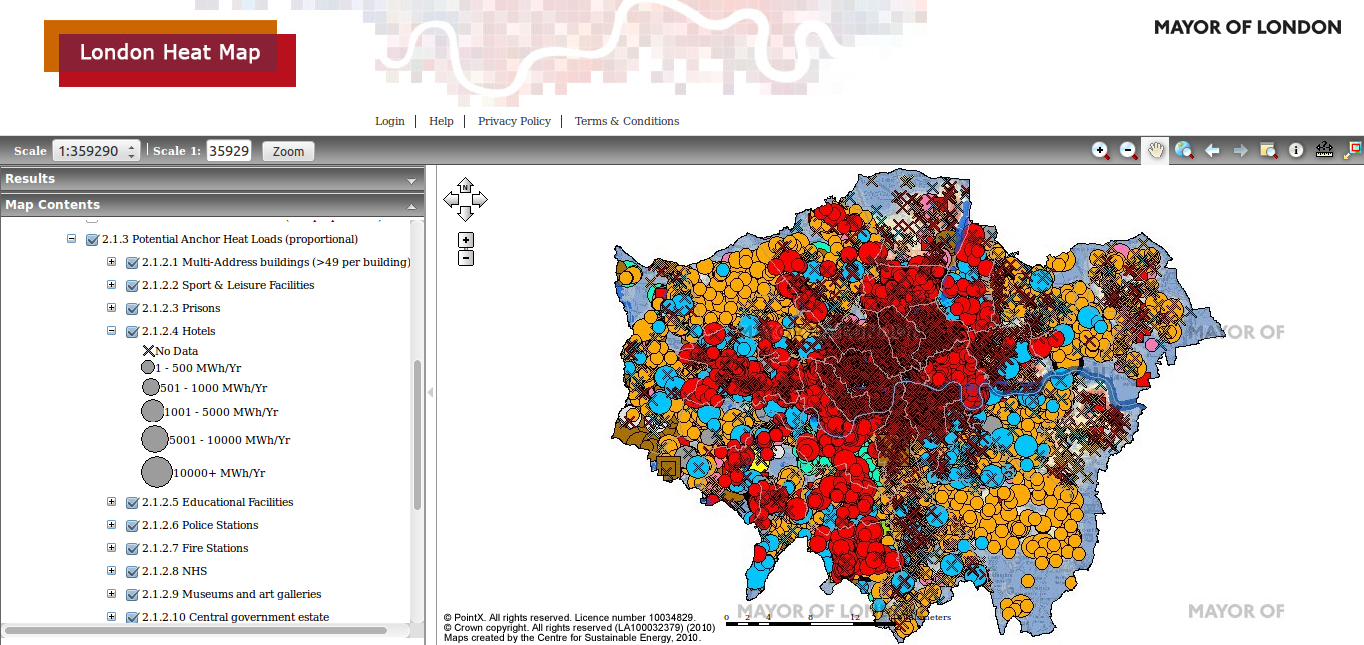
\includegraphics[width=0.7\linewidth]{londonHeatMapDmd.png}
  \caption[London Heat Map with Graduated Point Feature]{London Heat
    Map with Graduated Point Feature~\cite{londonHeatMapMap}}
  \label{fig:londonHeatMapDmd}
\end{figure}
~
\begin{figure}[h!]
  \centering
  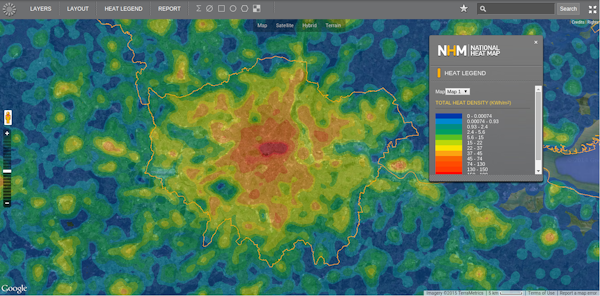
\includegraphics[width=0.7\linewidth]{nhm4London.png}
  \caption[National Heat Map for London]{National Heat Map that
    depicts the region of London~\cite{londonHeatMapMap}}
  \label{fig:nhm4London}
\end{figure}

Dutch heat map uses the same density map approach but the density is
not interpolated over space as in National Heat Map and EMIOFN. It is
represented as the height of the building or region.

The Lower Hill District Map does not directly represent energy demand
on the 3D map geometry, it uses an attribute table and bar chart to
visualize the demand quantity.

My dynamic energy map does not took the raster density map approach
because raster density map or graduated size symbol because the former
creates a 3D geometry layer and the latter create too much shape
distortion. Both approaches will impair my goal of representing a
realistic urban environment since the current map only contains one
map display window. These approaches could become valid in further
development of my current map so that it provide two side-by-side
window that shows the urban context and the energy demand layer in
different display window as in the example of National Heat Map
(\fref{fig:twoWindow}).

\begin{figure}[h!]
  \centering
  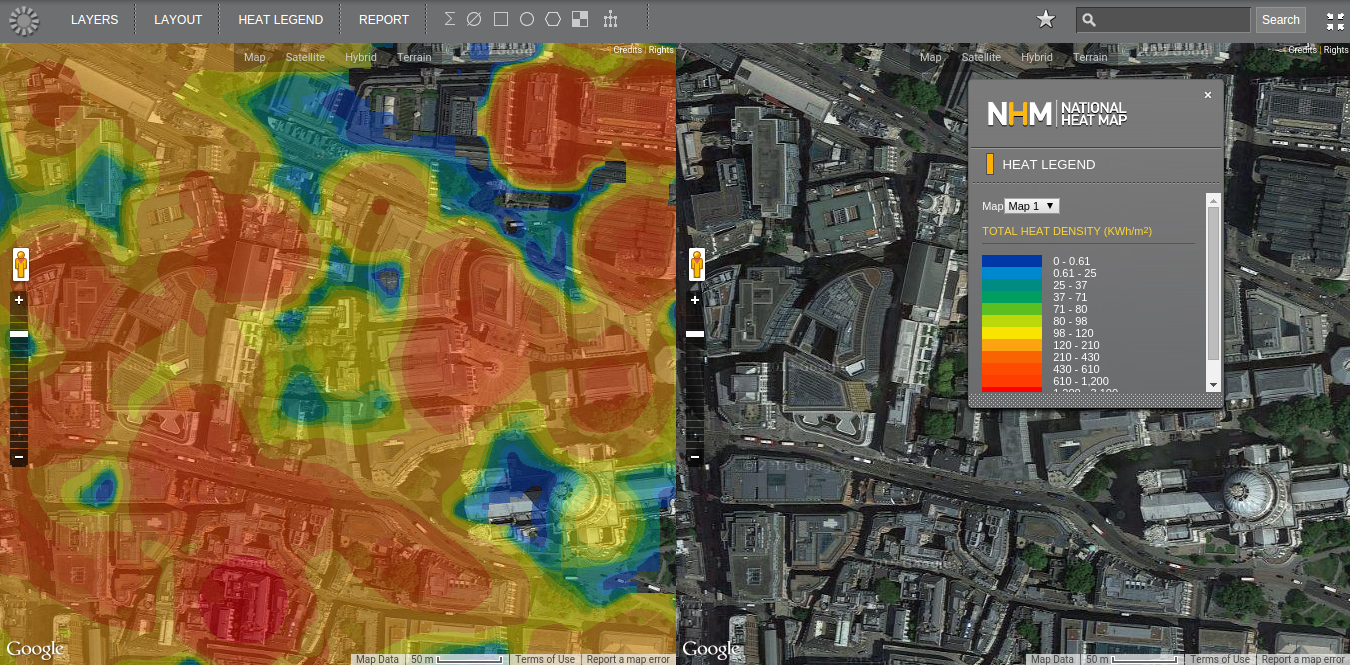
\includegraphics[width=0.7\linewidth]{twoWindow.png}
  \caption[Two Window Display of National Heat Map]{National Heat Map
    depicts the heating energy demand on the left and the urban
    environment context on the right~\cite{londonHeatMapMap}}
  \label{fig:twoWindow}
\end{figure}

\subsection{Techniques used}
The Calgary Map, Dutch Heat Map and EMIOFN map are stand-alone maps
produced with desktop GIS software. London Heat Map, National Heat
Map, Water Source Heat Map and Lower Hill District project are on-line
maps accessible through browsers. 

With limited software survey of ArcGIS and CityEngine, existing GIS
software are not capable of implementing an efficient dynamic energy
map. The major weakness is in the energy data visualization and the
high requirement of computational power. The limitations of existing
tools are summarized in \sref{sec:aggregateTime}. The tool used in the
implementation of the current dynamic energy map is
Python~\cite{python2015} with the Tkinter package~\cite{Tkinter2014}
for UI design and the pandas~\cite{pandas2015},
NumPy~\cite{NumPy2015}, Matplotlib~\cite{matplotlib2015} and
ggplot~\cite{ggplot2015} for database functions and data plot
creation. ImageMagick~\cite{ImageMagick2015} is used in image
formating and resizing. FFmpeg ~\cite{FFmpeg2015} is used in
connecting image sequences to animations.

\begin{table}[h!]
\centering
\caption{Map Technology Summary Table}
\label{tab:mapSummary}
\begin{tabular}{p{3cm}|p{3cm}|p{3cm}|p{3cm}}
  \hline
Project                 & Type    &             & Software                                  \\
  \hline
  \hline
London Heat Map         & Static  & web         & ArcGIS WebApp                             \\
  \hline
National Heat Map       & Static  & web         & Google Map API                            \\
  \hline
Water Source Heat Map   & Static  & web         & Google Map API                            \\
  \hline
Calgary Map             & Static  & stand-alone & ?                                         \\
  \hline
Dutch Heat Map          & Static  & stand-alone & ?                                         \\
  \hline
  \hline
Lower Hill District Map & Dynamic & web         & Map Creation: ArcScene, ArcMap, GIS Cloud \\
                        &         &             & Energy Simulation: EnergyPlus             \\
  \hline
EMIOFN                  & Dynamic & stand-alone & QGIS (Map Creation)                       \\
                        &         &             & HEM (Energy Simulation)                  \\
  \hline
\end{tabular}
\end{table}

\subsection{Building from the Lower Hill District Project}
My current work builds directly on the Lower Hill District Project. As
is mentioned in the introduction, the major functions of a dynamic
energy map is: holding, visualizing and analyzing community level high
spatial-temporal resolution energy demand and supply data and
connecting to simulation engine for dynamic performance analysis.

In the GIS map of the Lower Hill District Project by Baird et al.\
~\cite{baird2014}, holding spatial-temporal (although with low
temporal resolution) energy data and connecting to simulation software
is realized by processing the energy simulation data with Microsoft
excel and importing the csv file including ``building name, total
conditioned area annual, energy use intensity, annual and monthly peak
demand''. My dynamic energy map builds on this and makes the
geo-database hold more high resolution energy data imported from
EnergyPlus simulation, meaning the 8760 hourly energy data should be
contained in the dynamic energy map.

The feasibility analysis of a district energy system is performed in a
stand-alone Excel tool~\cite{baird2014}. My further improvement is to
aggregate part of the function of the screening tool, the calculation
and display of aggregated total heating and electricity demand, into
the dynamic energy map.

The spatial and temporal information are visualized separately in the
Lower District Hill Project: the spatial information of 3D building
geometry and location could be visually inspected in the GIS map but
not the hourly energy consumption information; the temporal
visualization of energy demand is done separately in the Excel
screening tool as 3D graphs, but no spatial context is present and the
spatial dimension is then lost. My improvement is to create a set of
spatial-temporal energy data display system that can better convey the
energy demand changes over space and time.